\chapter{METODOLOGI}
\label{bab:metodologi}

Bab ini menunjukkan bentuk uraian metodologi pada susunan enam bab. Prosedur contoh berfokus pada penyiapan dan pemeriksaan naskah. Tidak ada pengumpulan data atau eksperimen ilmiah yang dinyatakan telah dilaksanakan. Dalam skripsi pengguna, seluruh bagian berikut perlu diganti dengan prosedur yang memang digunakan untuk menjawab rumusan masalah.

\section{Rancangan}

Rancangan menerangkan hubungan antara tujuan, sumber informasi, prosedur, dan keluaran yang akan dianalisis. Penjelasan tersebut memungkinkan pembaca menilai apakah metode cukup untuk menghasilkan jawaban. Nama metode tidak cukup menjelaskan rancangan; pembaca juga memerlukan unit yang diamati, cara pemilihan unit, urutan perlakuan, serta aturan pemeriksaan.

Pada contoh penyusunan naskah, unit yang diperiksa adalah bagian dokumen, seperti judul, paragraf, tabel, gambar, persamaan, sitasi, dan lampiran. Setiap unit memiliki peran yang berbeda dalam penyampaian argumentasi. Prosedur diarahkan untuk memastikan peran tersebut terbaca dan hubungan antarbagiannya dapat ditelusuri melalui rujukan silang.

\section{Sumber dan Bahan}

Sumber pada naskah ini berupa dokumentasi resmi yang dirujuk dalam Bab \ref{bab:landasan}, sumber \LaTeX{} yang dapat disunting, serta keluaran dokumen yang perlu diperiksa. Ketiga kelompok tersebut mempunyai fungsi berbeda. Dokumentasi menerangkan kemampuan perangkat, sumber menyimpan isi dan penanda struktur, sedangkan keluaran memperlihatkan tampilan yang diterima pembaca.

Pada penelitian sesungguhnya, sumber dan bahan perlu dijelaskan menurut asal, cakupan, waktu, izin penggunaan, serta cara pemerolehan. Jika data diperoleh dari pihak lain, prosedur tidak boleh memberi kesan bahwa penulis mengumpulkannya secara langsung. Bila suatu bahan belum tersedia, kondisi itu perlu dilaporkan tanpa memperkirakan ukuran atau isinya.

\section{Tahapan}

Gambar \ref{fig:contoh-alur} menunjukkan urutan umum penyusunan contoh. Diagram dibuat dengan unsur vektor di dalam naskah sehingga tidak bergantung pada gambar dari berkas tambahan. Panah menjelaskan hubungan berurutan, bukan hubungan sebab-akibat ilmiah. Pada penelitian pengguna, nama tahap dan hubungan antarproses harus sesuai dengan metode yang benar-benar dikerjakan.

\begin{figure}[htbp]
  \centering
  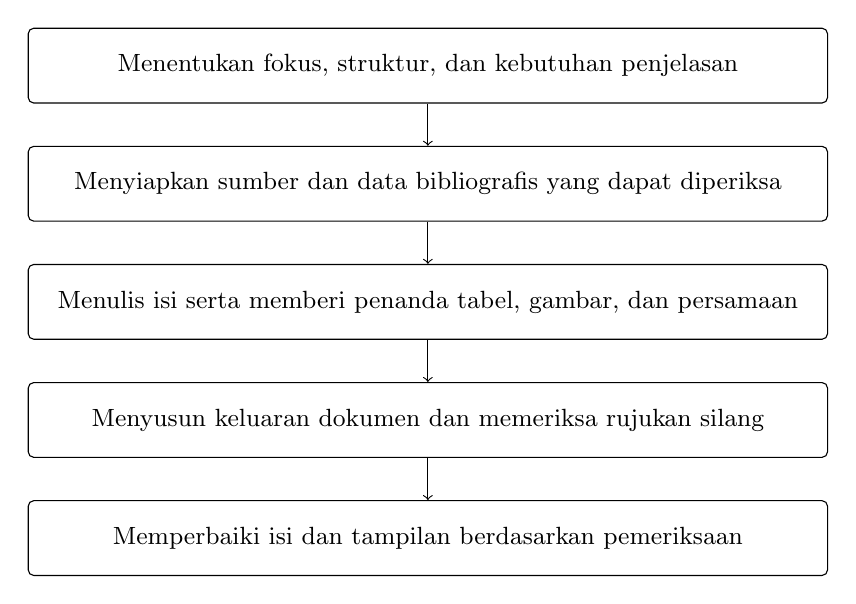
\begin{tikzpicture}[
    every node/.style={font=\small,align=center},
    tahap/.style={draw,rounded corners=2pt,text width=9.8cm,
      minimum height=0.95cm,inner sep=5pt}
  ]
    \node[tahap] (arah) at (0,0) {Menentukan fokus, struktur, dan kebutuhan penjelasan};
    \node[tahap] (sumber) at (0,-1.5) {Menyiapkan sumber dan data bibliografis yang dapat diperiksa};
    \node[tahap] (isi) at (0,-3.0) {Menulis isi serta memberi penanda tabel, gambar, dan persamaan};
    \node[tahap] (keluaran) at (0,-4.5) {Menyusun keluaran dokumen dan memeriksa rujukan silang};
    \node[tahap] (perbaikan) at (0,-6.0) {Memperbaiki isi dan tampilan berdasarkan pemeriksaan};
    \draw[->] (arah) -- (sumber);
    \draw[->] (sumber) -- (isi);
    \draw[->] (isi) -- (keluaran);
    \draw[->] (keluaran) -- (perbaikan);
  \end{tikzpicture}
  \caption{Contoh diagram alur penyusunan naskah}
  \label{fig:contoh-alur}
\end{figure}

\subsection{Penyiapan Struktur}

Struktur awal disusun berdasarkan kebutuhan argumentasi. Setiap bab mempunyai tujuan yang dinyatakan pada pengantar, kemudian dibagi menjadi bagian yang mendukung tujuan tersebut. Judul dan isi diperiksa bersama agar suatu bagian tidak memiliki nama yang lebih luas daripada materinya. Penulis dapat membuat garis besar sebelum mengembangkan paragraf, lalu memperbaikinya setelah hubungan antargagasan lebih jelas.

\subsection{Penulisan dan Penandaan Unsur}

Setiap unsur yang dirujuk diberi label yang bermakna. Label untuk gambar, tabel, persamaan, dan bab dibedakan melalui awalan, sehingga penulis dapat mengenali jenis rujukan ketika menyunting sumber. Penggunaan label membantu mempertahankan hubungan narasi dengan unsur yang dirujuk ketika posisi unsur atau nomor bab berubah.

\subsubsection{Pemeriksaan Penanda}

Penanda perlu unik dalam satu dokumen. Label yang sama pada dua unsur dapat membuat rujukan menunjuk unsur yang berbeda dari maksud penulis. Nama label sebaiknya menggambarkan isi dan tidak hanya mengikuti nomor yang dapat berubah. Pada contoh ini, Gambar \ref{fig:contoh-alur} tetap dirujuk melalui pengenal yang menjelaskan alurnya.

\subsection{Pemeriksaan Keluaran}

Pemeriksaan keluaran dilakukan setelah isi dan rujukan disusun. Pembaca keluaran perlu dapat melihat judul, awal dan akhir tabel, keterangan gambar, rumus, serta daftar referensi dengan jelas. Penulis juga memeriksa apakah unsur yang panjang tetap terbaca ketika berpindah halaman. Kriteria pemeriksaan contoh ditata pada Tabel \ref{tab:contoh-metode}.

\begin{table}[htbp]
  \centering
  \caption{Contoh hubungan tahap dan bahan pemeriksaan}
  \label{tab:contoh-metode}
  \begin{tabular}{p{3.2cm}p{4.0cm}p{5.0cm}}
    \toprule
    Tahap & Bahan yang dibaca & Pertanyaan pemeriksaan \\
    \midrule
    Struktur & Judul bab dan bagian & Apakah setiap bagian mempunyai fungsi yang jelas? \\
    Sumber & Sitasi dan bibliografi & Apakah identitas sumber sesuai dengan dokumen asal? \\
    Unsur & Tabel, gambar, persamaan & Apakah narasi menjelaskan unsur yang dirujuk? \\
    Keluaran & Dokumen terkompilasi & Apakah isi dan tampilan terbaca secara utuh? \\
    Perbaikan & Catatan pemeriksaan & Apakah perubahan menyelesaikan persoalan yang dicatat? \\
    \bottomrule
  \end{tabular}
\end{table}

\section{Penyajian dan Analisis}

Keluaran disajikan berdasarkan pertanyaan yang hendak dijawab. Unsur dengan sifat sebanding dapat ditempatkan dalam tabel, sedangkan hubungan tahapan dapat diperlihatkan melalui diagram. Informasi yang membutuhkan uraian alasan tetap disampaikan melalui paragraf. Pemilihan bentuk penyajian bertujuan mengurangi beban membaca tanpa menghilangkan kondisi dan batas bukti.

Pada penelitian sesungguhnya, analisis perlu dijelaskan sebelum hasil ditafsirkan. Jika digunakan ukuran numerik, definisi, arah makna, satuan, serta aturan penanganan kondisi khusus perlu ditulis. Jika analisis berupa pembacaan tematik, penulis perlu menerangkan unit, kategori, dan cara mengikat kategori dengan bukti. Metode yang ditulis harus memungkinkan pembaca memahami asal setiap hasil yang dilaporkan.

\section{Ketertelusuran}

Sumber naskah dan bahan pendukung disimpan dengan nama yang menunjukkan fungsi. Perubahan penting dicatat agar alasan perbaikan dapat ditemukan kembali. Pada template, pemisahan berkas per bab membantu pengguna menyunting bagian tertentu sambil mempertahankan satu berkas utama untuk penyusunan keseluruhan dokumen.

Penelitian dengan bahan yang tidak dapat dibagikan tetap memerlukan penjelasan tentang keberadaan dan batas akses bahan tersebut. Catatan ketertelusuran dapat menyertakan pengenal serta prosedur pemeriksaan tanpa mempublikasikan isi yang dibatasi. Lampiran \ref{lamp:contoh} memperlihatkan cara menata catatan pendukung secara umum; pengguna perlu menggantinya dengan informasi yang sesuai dengan penelitiannya.
